% "{'classe':('PSI'),'chapitre':'stat_pfs_2d','type':('td'),'titre':'Interface maître et esclave d\\'un robot', 'source':'CCP PSI 2015','comp':('B2-14','C1-05','C2-07'),'corrige':True}"
%\setchapterimage{bandeau}
\chapter*{TD \arabic{cptTD} :\\ 
Interface maître et esclave d'un robot  \ifnormal $\star$ \else \fi \ifdifficile $\star\star$ \else \fi \iftdifficile $\star\star\star$ \else \fi
 -- \ifprof Corrigé \else Sujet \fi}
\addcontentsline{toc}{section}{TD \arabic{cptTD} : 
Interface maître et esclave d'un robot  \ifnormal $\star$ \else \fi \ifdifficile $\star\star$ \else \fi \iftdifficile $\star\star\star$ \else \fi
 -- \ifprof Corrigé \else Sujet \fi}

\iflivret \stepcounter{cptTD} \else
\ifprof  \stepcounter{cptTD} \else \fi
\fi

\setcounter{question}{0}
\marginnote{CCP PSI 2015.}
\marginnote{
\UPSTIcompetence[2]{B2-14}
\UPSTIcompetence[2]{C1-05}
\UPSTIcompetence[2]{C2-07}
}

\begin{marginfigure}
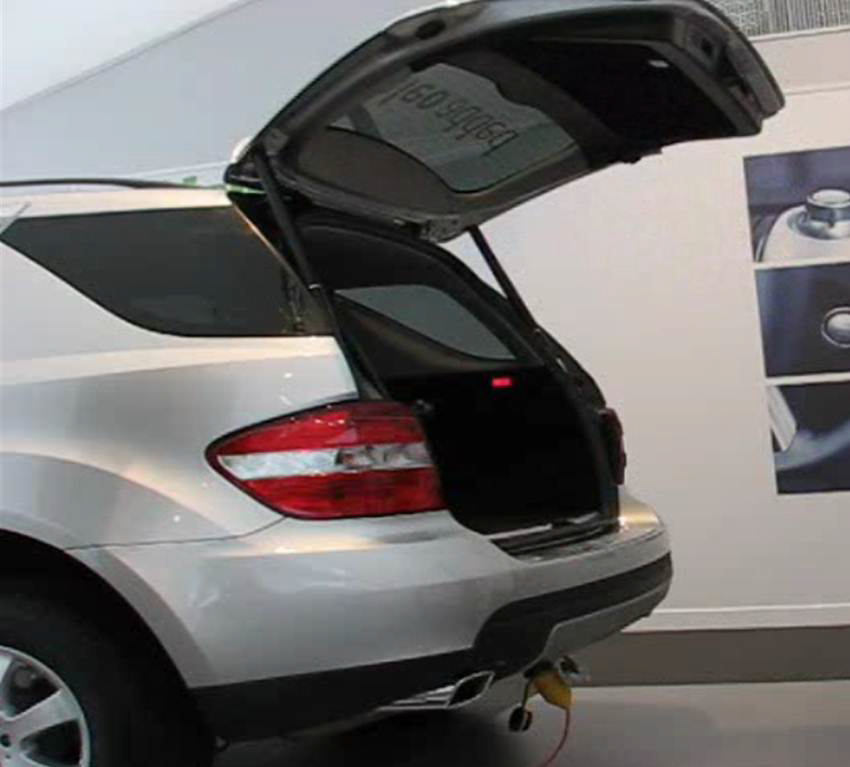
\includegraphics[width=\linewidth]{fig_00}
\end{marginfigure}


\section*{Mise en situation}
\ifprof
\else
La téléopération consiste à mettre en relation deux manipulateurs appelés communément
maître et esclave. Le manipulateur maître permet au chirurgien de donner sa consigne de
déplacement à l’aide d’un levier de commande tandis que l’esclave l’exécute au contact de
l’environnement (l’organe à opérer). Les deux sous-systèmes échangent des informations de
déplacement et d’effort au travers d’un ou plusieurs canaux de communication. Un retour
visuel est également mis en place en parallèle à ce dispositif.

\begin{marginfigure}
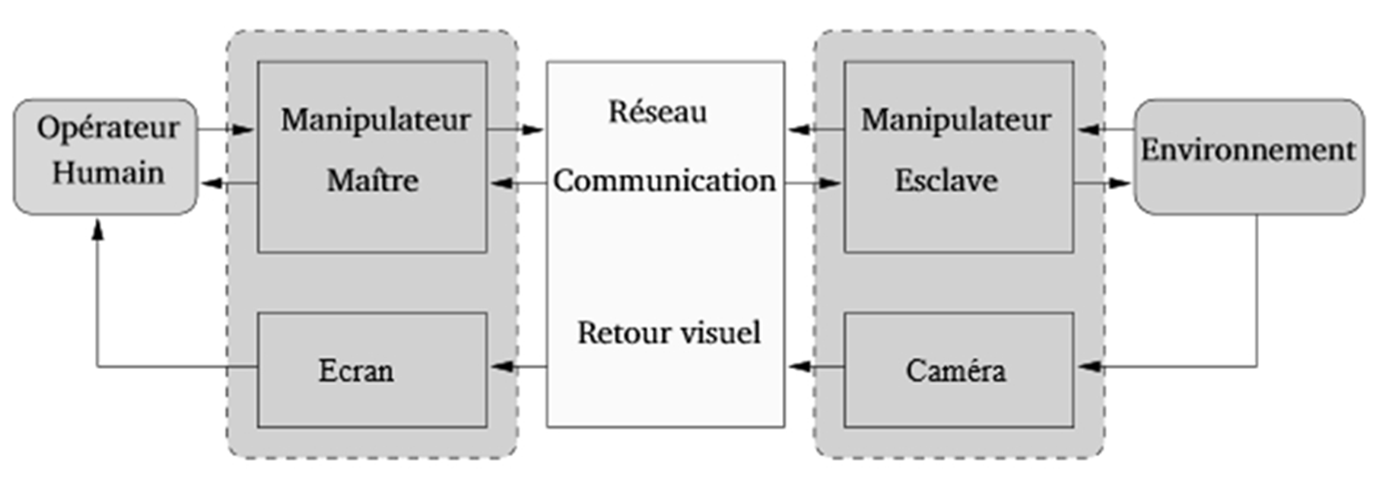
\includegraphics[width=\linewidth]{fig_00a}
%\textit{}
\end{marginfigure}
\fi

\section*{Modélisation de l’interface maître}
\ifprof
\else

Ce mécanisme est constitué de 4 barres reliées par des liaisons pivots.

\begin{marginfigure}
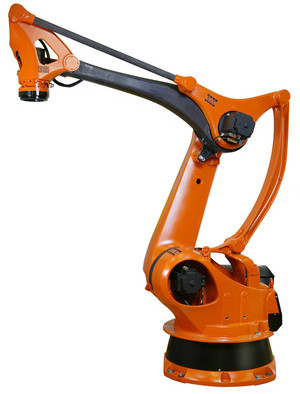
\includegraphics[width=\linewidth]{fig_01}
%\textit{}
\end{marginfigure}

\begin{obj}
Vérifier que l’exigence « Linéarité couple/effort » (id 1.3.2.2) peut être satisfaite
par le mécanisme de HOEKEN.
\end{obj}


\begin{marginfigure}
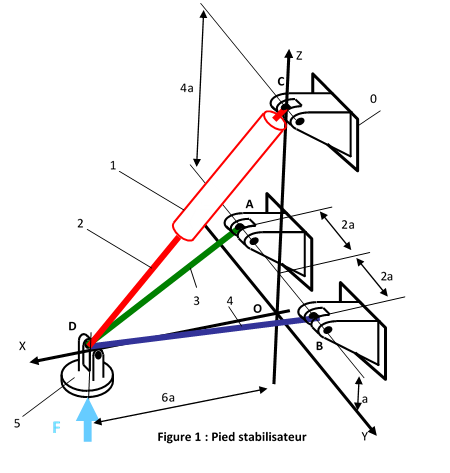
\includegraphics[width=\linewidth]{fig_02}
%\textit{}
\end{marginfigure}

\begin{itemize}
\item Solide $S_0$, repère $\rep{0}\repere{A}{x_0}{y_0}{z_0}$, $\vect{AB}=L_0\vect{x_0}$ avec $L_0 = \SI{50}{mm}$.
\item Solide $S_1$, repère $\rep{1}\repere{B}{x_1}{y_1}{z_0}$, $\vect{BC}=L_1\vect{x_1}$ avec $L_1 = \SI{25}{mm}$, $\theta_1=\angl{x_0}{x_1}=\angl{y_0}{y_1}$.
\item Solide $S_2$, repère $\rep{2}\repere{A}{x_2}{y_2}{z_0}$, $\vect{AD}=L_2\vect{x_2}$ avec $L_2 = \SI{62,5}{mm}$, $\theta_2=\angl{x_0}{x_2}=\angl{y_0}{y_2}$.
\item Solide $S_3$, repère $\rep{3}\repere{C}{x_3}{y_3}{z_0}$, $\vect{ED}=\vect{DC}=L_2\vect{x_3}$ avec  $\theta_3=\angl{x_0}{x_3}=\angl{y_0}{y_3}$.
\end{itemize}


\begin{itemize}
\item On notera $\torseurstat{T}{S_i}{S_j}=\torseurcol{X_{ij}}{Y_{ij}}{Z_{ij}}{L_{ij}}{M_{ij}}{N_{ij}}{P,\mathcal{B}_0}$ l'expression l’expression au point $P$, en projection dans la
base $\mathcal{B}_0$, du torseur de l’action mécanique exercée par le solide $S_i$ sur le solide $S_j$ ; toutes
les inconnues seront exprimées dans la base $\mathcal{B}_0$.
\item L’action mécanique exercée par le moteur sur $S_1$ sera modélisée par un couple $C_m(t) \vect{z_0}$.
\item L’action mécanique exercée par l’opérateur sur $S_3$ sera modélisée par une force $F(t) \vect{x_0}$
appliquée au point $E$.
\item L’accélération de la pesanteur sera négligée.%représentée par le vecteur $\vect{g}=-g\vect{z_0}$.
\item Les inerties des solides en mouvement et les frottements dans les guidages seront négligés.
\end{itemize}
\fi

\question{Réaliser le graphe d'analyse du mécanisme (liaisons et efforts).}
\ifprof
\begin{corrige}~\\

\begin{center}
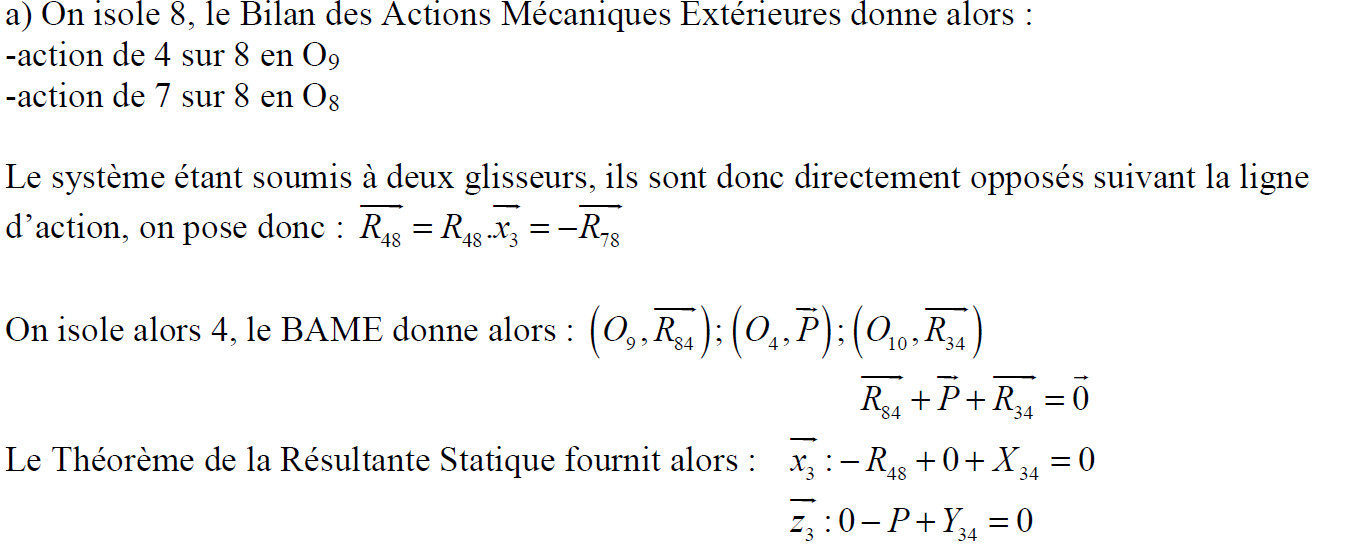
\includegraphics[width=.45\linewidth]{cor_01}
%\textit{}
\end{center}

\begin{center}
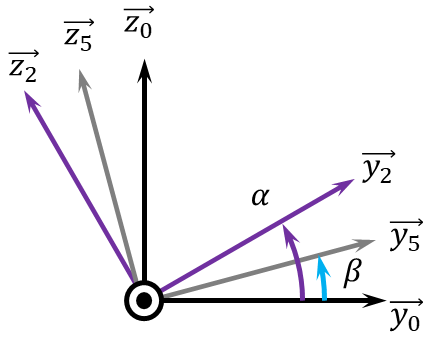
\includegraphics[width=.45\linewidth]{cor_02}
%\textit{}
\end{center}
\end{corrige}
\else
\fi


\ifnormal 

\question{\textbf{\#CCINP}
Déterminer les équations algébriques issues du développement des 4 relations suivantes :
\begin{itemize}
\item théorème du moment statique en $B$ appliqué à l’équilibre de $S_1$, en projection sur $\vect{z_0}$;
\item théorème du moment statique en $A$ appliqué à l’équilibre de $S_2$, en projection sur $\vect{z_0}$;
\item théorème du moment statique en $D$ appliqué à l’équilibre de $S_3$, en projection sur $\vect{z_0}$;
\item théorème de la résultante statique appliqué à l’équilibre de $S_3$, en projection sur $\vect{y_2}$.
\end{itemize}}
\ifprof
\begin{corrige}~\\
\end{corrige}
\else
\fi

\question{\textbf{\#CCINP}
Montrer que  :
$$C_m = \dfrac{L_1 F}{\sin \left(\theta_2 - \theta_3\right)}\left( \sin \theta_1 \sin\left( \theta_2+\theta_3 \right)  -2\cos \theta_1 \sin\theta_2\sin\theta_3\right).$$}
\ifprof
\begin{corrige}~\\
\end{corrige}
\else
\fi

\else
\fi


\ifdifficile


\question{\textbf{\#CCMP} Proposer une démarche permettant d'exprimer le couple moteur en fonction de l'effort de l'opérateur et des parmètres géométriques.}
\ifprof
\begin{corrige}~\\
\begin{itemize}
\item On commence par isoler le solide $S_2$ soumis à deux forces. D'après le PFS, on a donc $\torseurstat{T}{0}{2}=-\torseurstat{T}{3}{2}=\torseurl{F_{23}\vect{x_2}}{\vect{0}}{D}$.
\item Le solide $S_1$ est en rotation d'axe $\axe{B}{z_0}$. On réalise un TMS en $B$.
\item On isole $S_3$.Pour ne pas introduire les inconnues de liaison en $D$, on réalise un TMS en $D$.
\end{itemize}

\textbf{XP : à ce stade il manque une équation, on verra laquelle à la question suivante.}
\end{corrige}
\else
\fi
\else
\fi


\ifdifficile
\question{\textbf{\#CCMP} Mettre en \oe{}uvre cette démarche et montrer que
$$C_m = \dfrac{L_1 F}{\sin \left(\theta_2 - \theta_3\right)}\left( \sin \theta_1 \sin\left( \theta_2+\theta_3 \right)  -2\cos \theta_1 \sin\theta_2\sin\theta_3\right).$$}
\ifprof
\begin{corrige}~\\
Après avoir isolé $S_2$, on a vu que $\torseurstat{T}{2}{3}=\torseurl{F_{23}\vect{x_2}}{\vect{0}}{D}$.


\vspace{.5cm} 

On isole $S_1$.

On réalise le BAME.
\begin{itemize}
\item Action de la liaison pivot. 
\item Action du couple moteur.
\item Action de $S_3$ sur $S_1$ : $\torseurstat{T}{0}{1}=\torseurl{X_{31}\vect{x_0}+Y_{31}\vect{y_0}}{\vect{0}}{C}$. 
\end{itemize}

On applique le TMS en $B$ en projection sur $\vect{z_0}$ et on a : 

$C_m + \vect{BC}\wedge\left(X_{31}\vect{x_0}+Y_{31}\vect{y_0} \right) \cdot\vect{z_0}=0$

$\Leftrightarrow C_m + L_1\vect{x_1}\wedge\left(X_{31}\vect{x_0}+Y_{31}\vect{y_0} \right) \cdot\vect{z_0}=0$

$\Leftrightarrow C_m + L_1\left(-X_{31}\sin \theta_1+Y_{31} \cos \theta_1 \right) =0$


\vspace{.5cm} 

On isole $S_3$.

On réalise le BAME.
\begin{itemize}
\item Action de la liaison pivot en $C$ (1 sur 3). 
\item Action de la liaison pivot en $D$ (2 sur 3). 
\item Action de l'opérateur en $E$.
\end{itemize}

On applique le TMS en $B$ en projection sur $\vect{z_0}$ et on a : 

$\vect{DC}\wedge-\left(X_{31}\vect{x_0}+Y_{31}\vect{y_0} \right) +\left(\vect{DE}\wedge F(t)\vect{x_0} \right)\cdot\vect{z_0}=0$

$\Leftrightarrow\left( L_2\vect{x_3}\wedge-\left(X_{31}\vect{x_0}+Y_{31}\vect{y_0} \right) \right) \cdot\vect{z_0}-\left(L_2\vect{x_3}\wedge F(t)\vect{x_0}\right)\cdot\vect{z_0}=0$

$\Leftrightarrow L_2\left(X_{31} \sin \theta_3-Y_{31}\cos \theta_3 \right)  +L_2 F(t)\sin\theta_3=0$

À ce stade, il manque une équation pour éliminer $X_{31}$ ou $Y_{31}$. Il faut donc une équation de la résultante. Pour ne pas faire apparaître $F_{23}$, on peut isoler $S_3$ et réaliser un théorème de la résultante statique suivant $\vect{y_2}$ :

$\left(-\left(X_{31}\vect{x_0}+Y_{31}\vect{y_0} \right) +F_{23}\vect{x_2}+F(t)\vect{x_0}\right) \cdot \vect{y_2}=0$

$\Leftrightarrow -\left(- X_{31}\sin \theta_2+Y_{31}\cos\theta_2 \right)- F(t)\sin \theta_2=0$

$\Leftrightarrow  X_{31}\sin \theta_2-Y_{31}\cos\theta_2- F(t)\sin \theta_2=0$.

On a donc : 

$\left\{\begin{array}{l}
 C_m + L_1\left(-X_{31}\sin \theta_1+Y_{31} \cos \theta_1 \right) =0 \\
 L_2\left(X_{31} \sin \theta_3-Y_{31}\cos \theta_3 \right)  +L_2 F(t)\sin\theta_3=0 \\
 X_{31}\sin \theta_2-Y_{31}\cos\theta_2- F(t)\sin \theta_2=0
\end{array}
\right.
$

$\Leftrightarrow \left\{\begin{array}{l}
 C_m + L_1\left(-X_{31}\sin \theta_1+Y_{31} \cos \theta_1 \right) =0 \\
X_{31} \sin \theta_3-Y_{31}\cos \theta_3  + F(t)\sin\theta_3=0 \\
 X_{31} = \dfrac{Y_{31}\cos\theta_2+ F(t)\sin \theta_2}{\sin \theta_2}
\end{array}
\right.
$
%
%$\Leftrightarrow \left\{\begin{array}{l}
% C_m + L_1\left(-X_{31}\sin \theta_1+Y_{31} \cos \theta_1 \right) =0 \\
%\dfrac{Y_{31}\cos\theta_2+ F(t)\sin \theta_2}{\sin \theta_2} \sin \theta_3-Y_{31}\cos \theta_3   +F(t)\sin\theta_3=0 \\
% X_{31} = \dfrac{Y_{31}\cos\theta_2+ F(t)\sin \theta_2}{\sin \theta_2}
%\end{array}
%\right.
%$

$\Leftrightarrow \left\{\begin{array}{l}
 C_m + L_1\left(-X_{31}\sin \theta_1+Y_{31} \cos \theta_1 \right) =0 \\
Y_{31}\cos\theta_2\sin \theta_3+ F(t)\sin \theta_2 \sin \theta_3-Y_{31}\cos \theta_3\sin \theta_2   +F(t)\sin\theta_3\sin \theta_2=0 \\
 X_{31} = \dfrac{Y_{31}\cos\theta_2+ F(t)\sin \theta_2}{\sin \theta_2}
\end{array}
\right.
$

%$\Leftrightarrow \left\{\begin{array}{l}
% C_m + L_1\left(-X_{31}\sin \theta_1+Y_{31} \cos \theta_1 \right) =0 \\
%Y_{31}\left(\cos\theta_2\sin \theta_3-\cos \theta_3\sin \theta_2 \right)  =-2F(t)\sin \theta_2\sin\theta_3  \\
% X_{31} = \dfrac{Y_{31}\cos\theta_2+ F(t)\sin \theta_2}{\sin \theta_2}
%\end{array}
%\right.
%$



$\Leftrightarrow \left\{\begin{array}{l}
 C_m + L_1\left(-X_{31}\sin \theta_1+Y_{31} \cos \theta_1 \right) =0 \\
Y_{31}  =-2F(t)\dfrac{\sin \theta_2\sin\theta_3 }{\sin \left(\theta_3-\theta_2 \right)} \\
 X_{31} = \dfrac{Y_{31}\cos\theta_2+ F(t)\sin \theta_2}{\sin \theta_2}
\end{array}
\right.
$


$\Leftrightarrow \left\{\begin{array}{l}
 C_m + L_1\left(-X_{31}\sin \theta_1+Y_{31} \cos \theta_1 \right) =0 \\
Y_{31}  =-2F(t)\dfrac{\sin \theta_2\sin\theta_3}{\sin \left(\theta_3-\theta_2 \right)}  \\
 X_{31} = \dfrac{Y_{31}\cos\theta_2+ F(t)\sin \theta_2}{\sin \theta_2}
\end{array}
\right.
$

$\Leftrightarrow \left\{\begin{array}{l}
 C_m + L_1\left(-X_{31}\sin \theta_1+Y_{31} \cos \theta_1 \right) =0 \\
Y_{31}  =-2F(t)\dfrac{\sin \theta_2\sin\theta_3}{\sin \left(\theta_3-\theta_2 \right)}  \\
 X_{31} = -2F(t)\dfrac{\sin \theta_2\sin\theta_3}{\sin \left(\theta_3-\theta_2 \right)} \dfrac{\cos\theta_2}{\sin \theta_2}+ F(t) =F(t) \left(-2\dfrac{\cos\theta_2\sin\theta_3}{\sin \left(\theta_3-\theta_2 \right)} 
 +1\right)
\end{array}
\right.
$

On a donc 
$ C_m = L_1X_{31}\sin \theta_1- L_1Y_{31} \cos \theta_1 $ 
$ = -2F(t)\dfrac{\sin \theta_2\sin\theta_3}{\sin \left(\theta_3-\theta_2 \right)} L_1\sin \theta_1+ 2F(t)\dfrac{\sin \theta_2\sin\theta_3}{\sin \left(\theta_3-\theta_2 \right)}  L_1 \cos \theta_1 $ 

$ = 2F(t) L_1\dfrac{\sin \theta_2\sin\theta_3}{\sin \left(\theta_3-\theta_2 \right)}\left(-\sin \theta_1+  \cos \theta_1\right) $ 

\textbf{XP : je ne trouve pas la même expression que dans le sujet, je n'ai pas eu le temps de comprendre pourquoi.}


\end{corrige}
\else
\fi
\else
\fi

%$$C_m = \dfrac{L_1 F}{\sin \left(\theta_2 - \theta_3\right)}\left( \sin \theta_1 \sin\left( \theta_2+\theta_3 \right)  -2\cos \theta_1 \sin\theta_2\sin\theta_3\right).$$


%$$C_m = \dfrac{L_1 F}{\sin \left(\theta_2 - \theta_3\right)}\left( \sin \theta_1\sin \theta_2\cos\theta_3+\sin \theta_1\cos \theta_2\sin\theta_3  -2\cos \theta_1 \sin\theta_2\sin\theta_3\right).$$

Cette relation n’étant pas linéaire, on propose d’analyser les résultats d’une
simulation numérique en traçant le couple moteur/effort opérateur en fonction de l’abscisse du point $E$
%Q6.

\ifprof
\else
\begin{marginfigure}
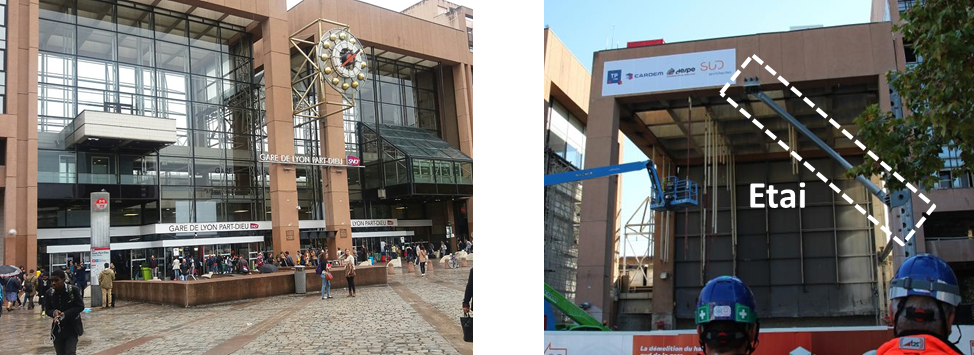
\includegraphics[width=\linewidth]{fig_03}
%\textit{}
\end{marginfigure}

\begin{marginfigure}
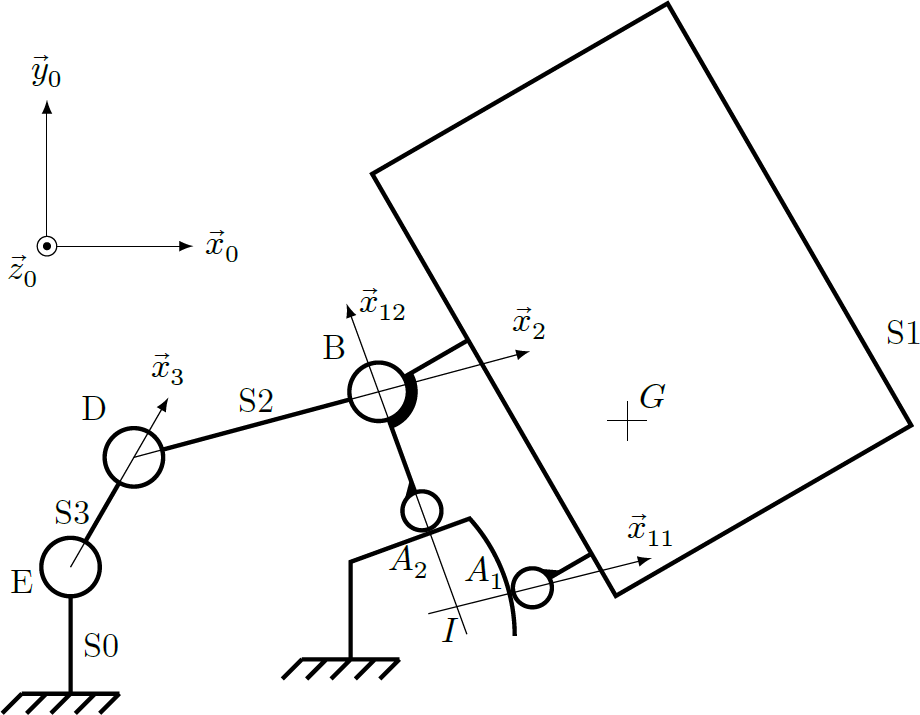
\includegraphics[width=\linewidth]{fig_04}
%\textit{}
\end{marginfigure}

\fi
\question{Retrouver ces graphes en utilsant Python. J'ai pas essayé, mais si eux ont réussi, pourquoi pas vous ? Il faut peut-être utiliser le premier devoir de vacances.}
\ifprof
\begin{corrige}~\\
\end{corrige}
\else
\fi


\question{Déterminer, à partir de la figure précédente, sur quel intervalle de l’abscisse $X_E$ l’exigence « Linéarité
couple/effort » (id 1.3.2.2) est satisfaite. (On ajoute que la course sur $X_E$ doit être supérieure à \SI{50}{mm}.)}
\ifprof
\begin{corrige}~\\
Pour un rapport $C_m/F$ de \SI{33,25}{mm}, la fourchette de 1\,\% est comprise entre \SI{32,9175}{mm} et \SI{33,5825}{mm}. La course de $X_E$ est donc de $20 - (-36)=\SI{56}{mm}$. L'exigence est vérifiée.
\end{corrige}
\else
\fi


%\ifprof
%\else
%\ifcolle
%\else
%\begin{marginfigure}[-4cm]
%\begin{solution}
%\begin{enumerate}
%\item \SI{2,34}{Nm}.
%\end{enumerate}
%\end{solution}
%\end{marginfigure}
%\fi
%\fi
%
